\documentclass[11pt,a4paper]{article}

\usepackage[utf8]{inputenc} 
\usepackage[T1]{fontenc} 
\usepackage{lmodern}
\usepackage[margin=2cm]{geometry}
\usepackage[german]{babel}
\usepackage{array}
\setlength{\parindent}{0pt}
\setlength{\parskip}{1ex plus 0.5ex minus 0.5ex}

\usepackage{amsmath} 
\usepackage{graphicx} 
\usepackage{booktabs}
\usepackage[colorlinks]{hyperref}
\usepackage{nicefrac}
\usepackage{gensymb}
\usepackage[usenames,dvipsnames,svgnames,table]{xcolor}
\usepackage{multirow}
\usepackage{tikz}
%\usepackage{chemfig}

\hbadness=99999
\newcommand\dif{\mathop{}\!\mathrm{d}}
\usepackage{etoolbox}

\makeatletter
\patchcmd{\@classz}
  {\CT@row@color}
  {\oldCT@column@color}
  {}
  {}
\patchcmd{\@classz}
  {\CT@column@color}
  {\CT@row@color}
  {}
  {}
\patchcmd{\@classz}
  {\oldCT@column@color}
  {\CT@column@color}
  {}
  {}
\makeatother
%\SetWatermarkText{\includegraphics[width=0.2\textwidth]{lol.gif}}
\begin{document}

{
\centering 
\large 
Physiklabor für Anf\"anger*innen \\
Ferienpraktikum im Sommersemester 2018 \\[4mm]
\textbf{\LARGE 
Versuch 36: Adiabatenexponenten
} \\[3mm]
(durchgef\"uhrt am 14.09.2018 bei Nico Strauß) \\
Andréz Gockel, Patrick M\"unnich, (Gruppe 14)\\
\today \\[10mm]
}
\vspace{55pt}
\tableofcontents

\pagebreak


\section{Ziel des Versuchs}

Das Ziel dieses Versuchs ist es, den Adiabatenexponenten von Luft und Argon zu bestimmen \footnote{Kohlenstoffdioxid war original teil des Experiments, wurde aber ausgelassen da nicht genügend Druck vorhanden war, um eine Schwingung zu erzeugen.}. Zuerst bestimmen wir aus den Strukturformeln von Stickstoff und Argon deren Molekularen Freiheitsgraden, welche verwendet werden, um den theoretischen Wert des Adiabatenexponentes herzuleiten. Um den Wert experimentell zu bestimmen, wird ein Versuchsaufbau nach Rüchardt-Flammerfeld \ref{JS1} verwendet, womit die Schwingungsdauer des Schwingkörpers gemessen wird. Leitet man die Formel \ref{F:0} her, die den Adiabatenexponent in Abhängigkeit der Schwingungsdauer bringt, kann man den dessen Wert bestimmen.


\section{Theoretische Bestimmung des Adiabatenexponenten}

Die Strukturformel für Stickstoff ist %\chemfig{\lewis{4, N}~\lewis{0, N}} 
und für Argon ist %\chemfig{\lewis{0246, Ar}} \ N$\equiv$N
Um den theoretischen Wert zu bestimmen verwenden wir diese Näherung für die Freiheitsgraden: $f = 3N-b$ \cite{Anleitung}, die bei diesen Gasen bei Raumtemperatur gilt. Wobei $N$ die Anzahl der Atome ist und $b$ die Anzahl der Bindungen.

Der Adiabatenexponent $\kappa$ ist definiert als $\kappa = \frac{c_p}{c_V}$, wobei $c_p$ die isobare Wärmekapazität ist und $c_V$ die isochore Wärmekapazität, welche durch Betrachtung der inneren Energie des Gases verallgemeinert werden können, womit wir $\kappa = \frac{f+2}{f}$ bekommen. Mit der Näherung haben wir $\kappa = \frac{3N-b+2}{3N-b}$. Für Stickstoff haben wir zwei Atome mit 3 Bindungen:
$$\kappa = \frac{6-3+2}{6-3} = \frac{5}{3}$$
und für Argon mit einem Atom und null Bindungen bekommen wir ebenfalls:
$$\kappa = \frac{3-0+2}{3-0} = \frac{5}{3}$$


\section{Experimentelle Bestimmung des Adiabatenexponenten}
\subsection{Aufbau}

Für dieses experiment haben wir einen Glaskolben den wir mit Luft bzw. Argon gas füllen, am Hals des Kolbens ist ein kleines Loch, welches für den Druckausgleich ist. Der Schwingkörper schwingt um dieses loch und die Anzahl der Schwingungen werden mit einem induktiven Ring gezählt. Wir können das einströmen von Gas durch ein Feinventil regulieren. Es muss ständig etwas Gas einströmen da der Schwingkörper sonst durch Reibung abgebremst werden würde.  

\begin{figure}[h]
\centering
\fbox{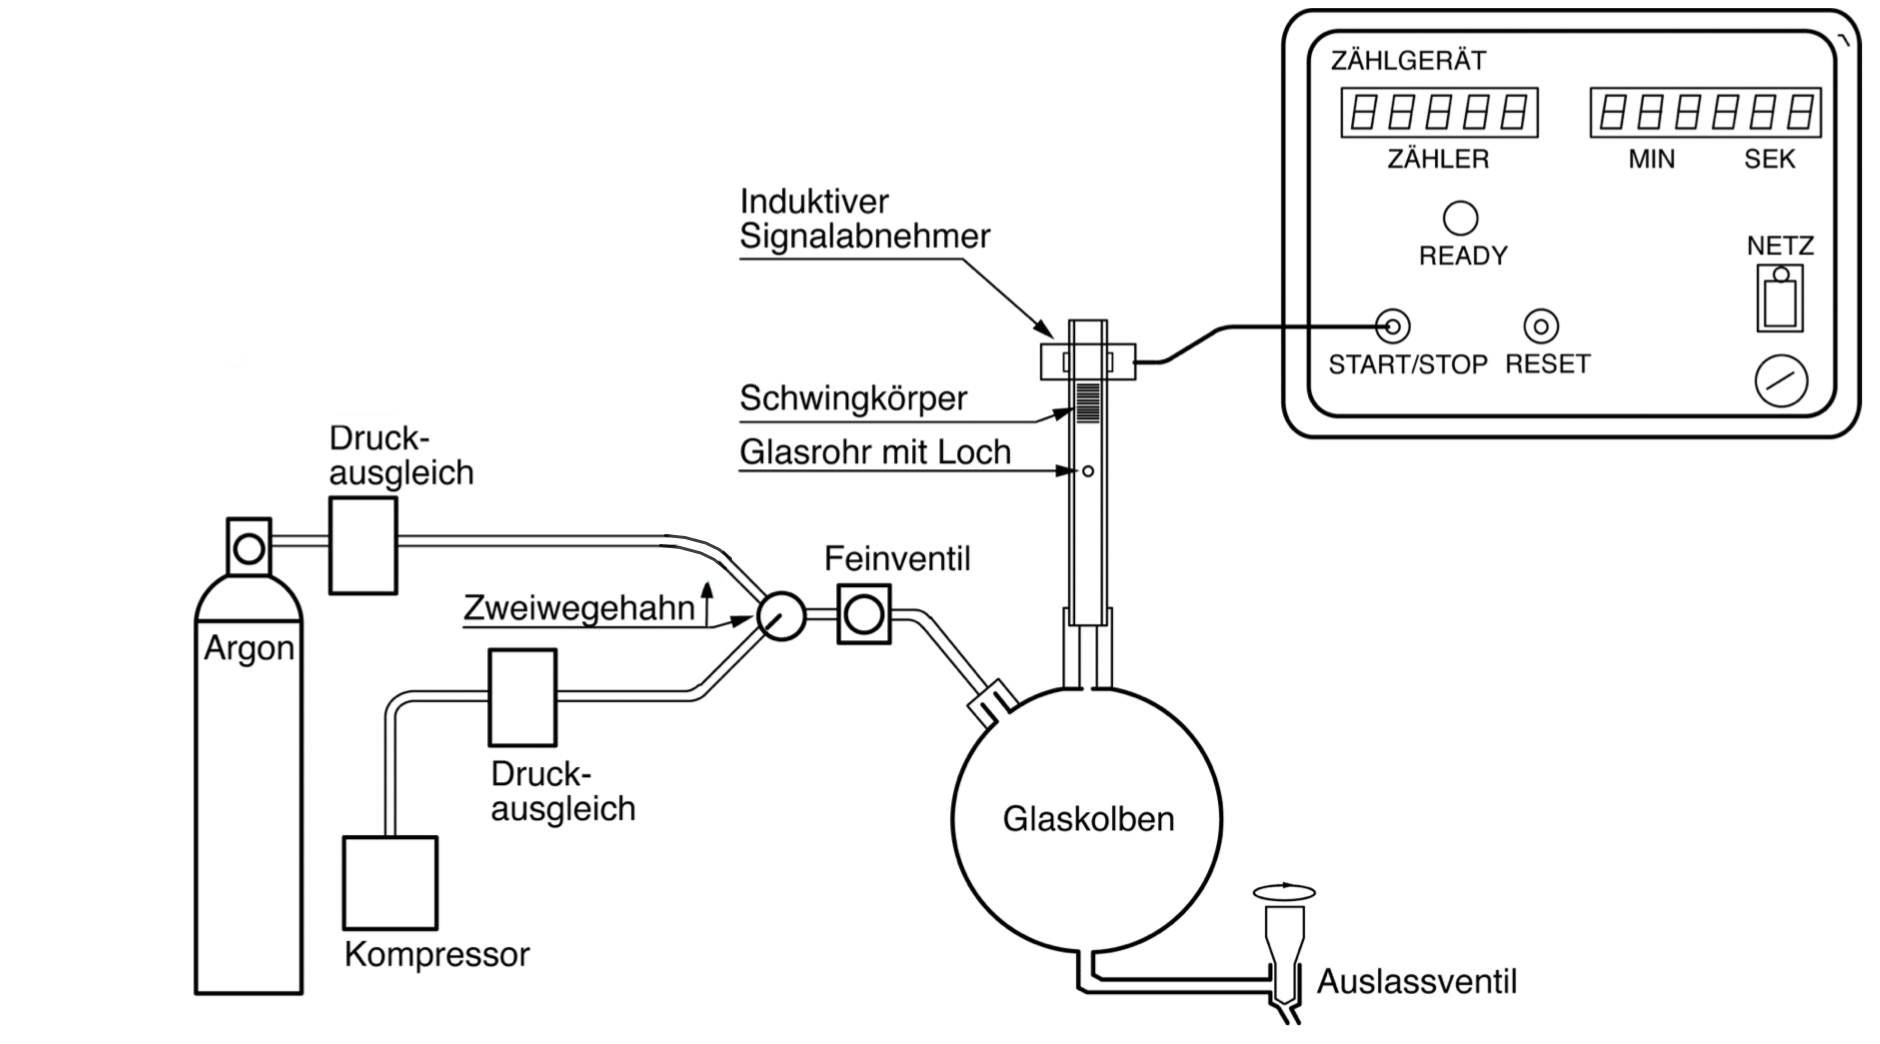
\includegraphics[width=0.8\textwidth]{auuufbauuu}}
   \renewcommand\thefigure{B1}
\caption[Versuchsaufbau]{Versuchsaufbau \cite{Anleitung}}
\label{JS1}
\end{figure}

\subsection{Durchführung}

Bevor wir mit den Messungen anfangen können müssen wir sicher sein dass, das Gas in dem Kolben rein ist. Hierfür öffnen wir das Auslassventil und wir lassen die Luft für eine Minute durch den Kolben fließen. Anschließend schliessen wir das Auslassventil und benutzen das Feinventil um eine geringe Strömung zu bekommen die unser Schwingkörper in Schwingung versetzt. Wir schalten dann das Messgerät für 1000 Schwingungen an und schreiben für alle 200 Schwingungen die zeit auf. Zum vergleich schauen wir uns 5 mal 100 Schwingungen an und schreiben diese Zeiten auf. 

Demnach schalten wir den Zweiweghahn auf Argon um und öffnen das Auslassventil für 5 Minuten. Die Messungen für Argon liefen genau so ab wie für Luft. 

\subsection{Theorie}

Zur experimentellen Bestimmung des Adiabatenexponentens benutzen wir

\begin{equation}
T=\frac{2\pi}{\omega}=2\pi\sqrt{\frac{mV}{q^2p\kappa}}\label{eqT1}
\end{equation}

mit $m$ als die Masse und $V$ das Volumen des Gases. $q$ ist die Fl\"ache des Glasrohrs, $p$ der Druck und $\kappa$ ist der gesuchte Adiabatenexponent. Au\ss erdem ist $\omega$ hier die Frequenz und $T$ die Periodendauer. Diese Formel wird dann zu

\begin{equation}
\kappa=4\pi^2\frac{mV}{q^2pT}\label{eqT2}
\end{equation}

umgeschrieben.

Die Formel (\ref{eqT2}) stammt aus der folgenden Herleitung:
%pV^\kappa=const.\textrm{ mit }\kappa=\frac{c_p}{c_v}\\
%pV=\frac{k_BNT}{V}\\
%C_P=\frac{1}{n}\frac{\dif Q}{\dif T}|_{p=const.}\\
%C_V=\frac{1}{n}\frac{\dif Q}{\dif T}|_{V=const.}\\
%\dif U=hC_V\dif T\\
%\dif U=nC_P\dif T-p\dif V\\
%nD_V\dif T=nC_P\dif T-p\dif V\\
$$F=q\dif p\\
$$
$$V=qx\Rightarrow \dif V=q\dif x\\
$$
$$\Rightarrow \dif F=q\dif x=\frac{-pq^2\kappa\dif x}{V}\\
$$
$$F=m\ddot{x}\Rightarrow \omega^2=\frac{pq^2\kappa}{mV}
$$

$F$ steht f\"ur die auf den K\"orper wirkende Kraft und $x$ die Auslenkung.

Die Fehler von $n$ und $T$ werden mit

\begin{equation}
s_n=\sqrt{n}\label{equn}
\end{equation}

f\"ur $n$ Schwingungen und

\begin{equation}
s_T=\frac{1}{\sqrt{n}}\overline{T}\label{equt}
\end{equation}

f\"ur die Periodendauer $T$ mit $n$ Schwingungen durchgef\"uhrt.

\subsection{Auswertung und Fehleranalyse}

%Zur Erleichterung der Berechnungen wurden zuerst die Werte für $A$, $p$ und deren Unsicherheiten berechnet. 
%
%Die Unsicherheiten von $A$ lassen sich mit der vereinfachten Formel für Produkte und Quotienten bestimmen:

Zur Berechnung der Fehler nehmen wir folgende Formel f\"ur Produkte  und Quotienten zunutze:
\begin{equation}
\left\vert\frac{\Delta z}{z_0}\right\vert = \sqrt{\left({a\frac{\Delta x}{x_0}}\right)^2+\left({b\frac{\Delta y}{y_0}}\right)^2} \ \ \textrm{f\"ur } z=x^a y^b. 
\end{equation}

Damit berechnen wir unseren Fehler f\"ur die Fl\"ache q
\[
\left\vert\frac{\Delta q}{q}\right\vert=2\frac{\Delta\nicefrac{D}{2}}{\nicefrac{D}{2}}
\]
mit Durchmesser $D=(13.5\pm0.3)\,$mm$^2$.
%und deshalb ist
%$$ A = (1,517 \pm 0,001) \cdot 10^{-4} \textrm{m}^3$$
%Für $p$ wurden zuerst die Unsicherheiten von $p_S$ mit der obigen Formel berechnet und danach mit der Formel für Summen berechnet, nämlich:
Um unser $p$ zu berechnen nutzen wir erstmals die gleiche Formel f\"ur unser $p_S=\nicefrac{F}{q}$ und erhalten
\[
\left\vert\frac{\Delta p_S}{p_S}\right\vert=\sqrt{\left(\frac{\Delta F}{F}\right)^2+\left(-1\frac{\Delta q}{q}\right)^2}
\]
Da der Druck f\"ur die Rechnung aus der Summe vom Au\ss endruck und dem Innendruck besteht brauchen wir noch die Formel f\"ur Summen:
\begin{equation}
\Delta z = \sqrt{(a\Delta x)^2 + (b \Delta y)^2+\ldots} \textrm{  f\"ur } z = ax+by+\ldots.
\end{equation}
Hiermit erhalten wir:
\[
\left\vert\frac{\Delta p}{p}\right\vert=\sqrt{\Delta p_S+\Delta p_A}
\]

%Und endlich können die Unsicherheiten für $\kappa$ mit der Formel (2) berechnet werden. Aber da die Beträge von $\frac{\Delta V}{V}$ und $\frac{\Delta T_S}{T_S}$ überwiegend größer waren als die Beträge der anderen Terme, wurden nur diese zwei Terme berücksichtigt. 

%Die Unsicherheit von $\kappa$ lässt sich deshalb schreiben als:
Da f\"ur $\kappa$ mehrere aufgrund vergleichbar niedrige Werte vernachl\"assigbare Terme vorhanden sind, k\"onnen wir einfach mit der Folgenden Gleichung rechnen:
\begin{equation}\Delta \kappa  = \kappa \sqrt{\left({\frac{\Delta V}{V}}\right)^2 + \left({2\frac{\Delta T_S}{T_S}}\right)^2} \end{equation}

Die gemessen Werte der Variablen au\ss erhalb von der Anzahl Schwingungen und der Zeit sind:
\begin{itemize}
\item $m=(5.7\pm0.3)\,$g
\item $V=(2.225\pm0.005)\,$cm$^3$
\item $q=(14.3\pm0.06)\,$cm$^2$
\item $p_a=(988\pm1)$\,mbar
\end{itemize}

Mit unseren Messwerten, welche im Anhang gefunden werden k\"onnen, und (\ref{eqT2}) bekommen wir folgende Werte f\"ur Luft und Argon mit 100 Schwingungen:

\begin{table}[h]
\centering
\renewcommand\thetable{T1}
\caption{Adiabatenexponente}
\vspace{11pt}
\begin{tabular}{ccc}
\toprule
Messreihe & $\kappa$ Luft &  $\kappa$ Argon\\
\midrule
1 & 1.6(4) & 1.9(4)\\
2 & 1.6(4) & 1.9(4)\\
3 & 1.6(4) & 1.9(4)\\
4 & 1.6(4) & 1.9(4)\\
5 & 1.5(4) & 1.9(4)\\
\bottomrule 
\end{tabular}
\label{tab:B1}
\end{table}

\pagebreak

F\"ur 1000 Schwingungen sehen die Werte folgenderma\ss en aus:

\begin{table}[h]
\centering
\renewcommand\thetable{T1}
\caption{Adiabatenexponente}
\vspace{11pt}
\begin{tabular}{ccc}
\toprule
Messreihe & $\kappa$ Luft &  $\kappa$ Argon\\
\midrule
1 & 1.6(2) & 1.8(2)\\
2 & 1.6(2) & 1.9(2)\\
\bottomrule 
\end{tabular}
\label{tab:B1}
\end{table}

\subsection{Diskussion}

Um unsere Ergebnisse leicht zu vergleichen, bilden wir erstmal die Mittelwerte f\"ur $\kappa$. Die Formel f\"ur die Fehlerberechnung des Mittelwerts lautet:

\begin{equation}
s_x=\sqrt{\frac{1}{n-1}\sum_{i=1}^n(x_i-\overline{x})^2}.\label{uncertainty1}
\end{equation}

Somit erhalten wir als Mittelwerte f\"ur den gemessenen Adiabatenexponent von Luft $1.59\pm0.1$ und f\"ur Argon $1.87\pm0.1$.

Mithilfe der Formel

\begin{equation}
t=\frac{|x_0-y|}{u_x}\label{abw}
\end{equation}

und den Werten von der theoretischen Berechnung und der Messung bekommen wir $t=0.63$ f\"ur Luft und $t=1.53$ f\"ur Argon. Beide dieser Werte liegen innerhalb des erw\"unschten $t<2$ Bereichs. Dies bedeutet, dass diese Werte als vertr\"aglich gelten.

Zum Verbessern der Versuchsdurchf\"uhrung h\"atte man nach \"Anderung des Gases lange aussp\"ullen k\"onnen. Zwar wurde f\"ur f\"unf Minuten gesp\"ul, indem man das Gas durch den ge\"offneten Kolben laufen lie\ss , jedoch ist es durchaus m\"oglich, dass der Kolben trotzdem nicht vollkommen Durchgesp\"ult wurde. Zudem kommt, dass das Gas innerhalb der Gasflasche eventuell auch andere Gase beinhaltet.

Dazu kommt, dass sich der Au\ss endruck leicht \"andern kann, da der Raum nicht abgeschlo\ss en war. Ge\"offnete T\"uren und Fenster k\"onnen eventuell den Druck \"andern. Dies ist jedoch nicht sehr Einflussreich, da der Au\ss endruck sich nicht sehr stark ge\"andert haben wird.

\vfill

\begin{thebibliography}{9}
% \bibitem{Uncertainties}''Correlations between variables are automatically handled, which sets this module apart from many existing error propagation codes.'' - https://pythonhosted.org/uncertainties/
 \bibitem{Anleitung} Physikalisches Institut der Albert-Ludwigs-Universität Freiburg (Hrsg.) (08/2018): Versuchsanleitungen zum Physiklabor für Anfänger*innen, Teil 1, Ferienpraktikum im Sommersemester 2018.
 \end{thebibliography}
%Systematische und statistische Fehler.

\pagebreak


\section{Anhang}


%\begin{table}[h]
%\centering
%\renewcommand\thetable{T1}
%\caption{Messwerte}
%\vspace{11pt}
%\rowcolors{2}{gray!10}{white}
%\begin{tabular}{|>{\columncolor[gray]{1}}c|r|r|r|}
%\multicolumn{2}{c}{}&\multicolumn{1}{c}{Luft} & \multicolumn{1}{c}{Argon}\\
%\hline
%Messreihe & Periode & Zeit in $s$ & Zeit in $s$\\
%\hline 
%&200$\pm14$  & 78.53  &  75.06 \\
%&400$\pm20$  & 156.89 & 149.50 \\
%&600$\pm25$  & 235.78 & 223.57 \\
%&800$\pm28$  & 314.35 & 297.25 \\
%\multirow{-5}{*}{1}
%&1000$\pm32$ & 392.34(13) & 371(5) \\ 
%\hline
%&200$\pm14$  & 78.44  &  73.03 \\
%&400$\pm20$  & 156.87 & 145.91 \\
%&600$\pm25$  & 235.38 & 218.79 \\
%&800$\pm28$  & 313.95 & 291.47 \\
%\multirow{-5}{*}{2}
%&1000$\pm32$ & 392.52(13) & 364(5) \\ 
%\hline
%&100$\pm10$ & 39.1(4) & 36.10(4) \\
%&100$\pm10$ & 39.0(4) & 36.18(4) \\
%&100$\pm10$ & 39.2(4) & 36.14(4) \\
%&100$\pm10$ & 39.0(4) & 36.10(4) \\
%\multirow{-5}{*}{3}
%&100$\pm10$ & 40.0(4) & 36.16(4) \\ 
%\hline
%\end{tabular}
%\label{tab:B1}
%\end{table}
%

\begin{table}[h]
\centering
\renewcommand\thetable{T1}
\caption{Messwerte}
\vspace{11pt}
\rowcolors{2}{gray!10}{white}
\begin{tabular}{crrr}
\multicolumn{2}{c}{}&\multicolumn{1}{c}{Luft} & \multicolumn{1}{c}{Argon}\\
\toprule
Messreihe & Periode & Zeit in $s$ & Zeit in $s$\\
\midrule
1&1000$\pm32$ & 392.34(13) & 371(5) \\ 
2&1000$\pm32$ & 392.52(13) & 364(5) \\ 
\hline
3&100$\pm10$ & 39.1(4) & 36.10(4) \\
4&100$\pm10$ & 39.0(4) & 36.18(4) \\
5&100$\pm10$ & 39.2(4) & 36.14(4) \\
6&100$\pm10$ & 39.0(4) & 36.10(4) \\
7&100$\pm10$ & 40.0(4) & 36.16(4) \\ 
\bottomrule
\end{tabular}
\label{tab:B1}
\end{table}

\phantom{lol}
\end{document}